\section{Framework}

% === OVERVIEW ===================================

\begin{frame}
\frametitle{Overview}
	\begin{itemize}
		\item<+-> Shallow dense neural network \& supervised learning
		\item<+-> Goal: Learning the SR i.e., a transition probability matrix
		\item<+-> Two configurations were tested
		\begin{enumerate}
			\item<+-> Artificial rules with manufactured data set (``First model'')
			\item<+-> Self derived rules and data set (``Word to word model'')
		\end{enumerate}
		\item<+-> Rule: word pair consisting of a predecessor and successor word serving as input and output
		\item<+-> In case of word to word models: Data was collected from two books (german \& english)
		\item<+-> The quality of the learned rules determines the SR
	\end{itemize}
\mynote{
\begin{itemize}
    \item[ü] Starting with a general overview
	\item For training a shallow dense neural network with $ 1 $ layer was trained with supervised learning.
	\item The goal was to learn a SR for $ t=0 $ which equals a transition probability matrix.
	\item Two configurations were tested
    \begin{itemize}
		\item One having artificial rules with a manufactured data set, called``First model''...
        \item the other works with self derived rules and data set, called ``Word to word model''
    \end{itemize}
	\item A ``Rule'' is a word pair consisting of a predecessor and successor word serving as input and output
	\item In case of word to word models: Data was collected from two books in german \& english respectively
    \item The quality of the learned rules determines the Successor representation
\end{itemize}
}
\end{frame}

% === FIRST MODEL ===================================

\begin{frame}{First model}
	\begin{itemize}
		\item<1-> Cognitive room consists of all words used for training
		\item<2-> Data was generated by made up rules like {\huge \texttt{Verb → Adjective}} using \onehot{s}
		\item<3-> The single predictions after training describe the transition probability matrix
		\item<4-> This type of model is tailored and clear
	\end{itemize}
	\vfill
   	\begin{figure}
   		\centering
   			\includegraphics<2->[scale=0.5]{Bilder/first_model_graph2}
   	\end{figure}
% --------------------------------------
\mynote{
\begin{itemize}
    \item[ü] I start with the details of the First Model
	\item The cognitive room consists of all words used for training which is basically a list containing all words
	\item The data was generated by made up rules like {\huge \texttt{Verb → Adjective}}, the concrete words were chosen randomly and converted to \onehot{s} by denoting a one at the index in the cognitive room
	\item[i] In the picture there is simple scenario depicted. The rules can be combined to a graph. The gray vectors resemble the word and in this case the cognitive room has $ 3 $ elements.
    \item The single predictions after training describe the transition probability matrix
    \item This type of model is tailored and clear
\end{itemize}
}
\end{frame}

% === WORD TO WORD MODEL 1/2 ===================================

\begin{frame}
\frametitle{Word to word model}
	\begin{itemize}
		\item<+-> In principle similar to the first model approach
		\item<+-> But rules and data derived from real language examples
		\item<+-> Books were parsed using techniques from Natural Language Processing (via {\huge \texttt{spacy}})
		\begin{itemize}
			\item<+-> In german and english, because the former's word order is more variable $ \to $ may cause troubles
		\end{itemize}
	\end{itemize}
\Os{5}{
	\begin{columns}
		\begin{column}{0.375\textwidth}
				\vspace*{4.5cm}\\
				\hspace{15mm}\textbf{Alice sends Bob} a message.\hspace{10mm}$ \Longrightarrow $
		\end{column}
	%
		\begin{column}{0.625\textwidth}
			\begin{figure}
				\centering % TODO Bild ohne Kante einfügen
				\includegraphics<5->[scale=0.39]{Bilder/w2w_small}
			\end{figure}
		\end{column}
	\end{columns}
}
% --------------------------------------
\mynote{
\begin{itemize}
    \item[ü] Now, word to word models, which...
	\item ... are in principal similar to the first model approach
	\item But rules and data were derived from real language examples
	\item To do so, books were parsed using techniques from Natural Language Processing and provided via the python module \spacy. The techniques used will be demonstrated shortly.
    \begin{itemize}
        \item In german and english, because the former's word order is more variable, this may cause trouble
    \end{itemize}
    \item[i] SATZ UND GRAPH ZEIGEN
	\item As little example: The sentence ``Alice sends Bob a message.'' is tokenized (this means words become objects with additional information), lemmatized (this stands for mapping conjugated verbs onto infinitives) and finally coupled to have a rule, as we can see in the graph on the right. The middle vertex is annotated (on purpose) with ``send'' not ``sends'' due to lemmatization. Each edge encodes a rule with input and output word.
\end{itemize}
}
\end{frame}

% === WORD TO WORD MODEL 2/2 ===================================

\begin{frame}
\frametitle{Word to word model}
	\begin{itemize}
		\item In principle similar to the first model approach
		\item But rules and data derived from real language examples
		\item<+-> Books were parsed using techniques from Natural Language Processing (via {\huge \texttt{spacy}})
		\begin{itemize}
			\item In german and english, because the former's word order is more variable $ \to $ may cause troubles
		\end{itemize}
	\end{itemize}
	\begin{columns}
		% SPALTE 1
		\begin{column}{0.375\textwidth}
			% SPALTE 1.1
			\begin{column}{0.85\columnwidth}
				\vspace*{3.7cm}\\
				\hspace{7.5mm}\parbox{0.85\columnwidth}{\textbf{Alice sends Bob} a message. [...] \textbf{Alice goes} to the grocery store. [...]. Peter \textbf{sent him} a letter. [...] \textbf{Bob went} to his friend.}
			\end{column}
			% SPALTE 1.2
			\begin{column}{0.15\columnwidth}
				\vspace*{4.5cm}\\
				$ \Longrightarrow $
			\end{column}
		\end{column}
		% SPALTE 2
		\begin{column}{0.625\textwidth}
			\begin{figure}
				\centering
				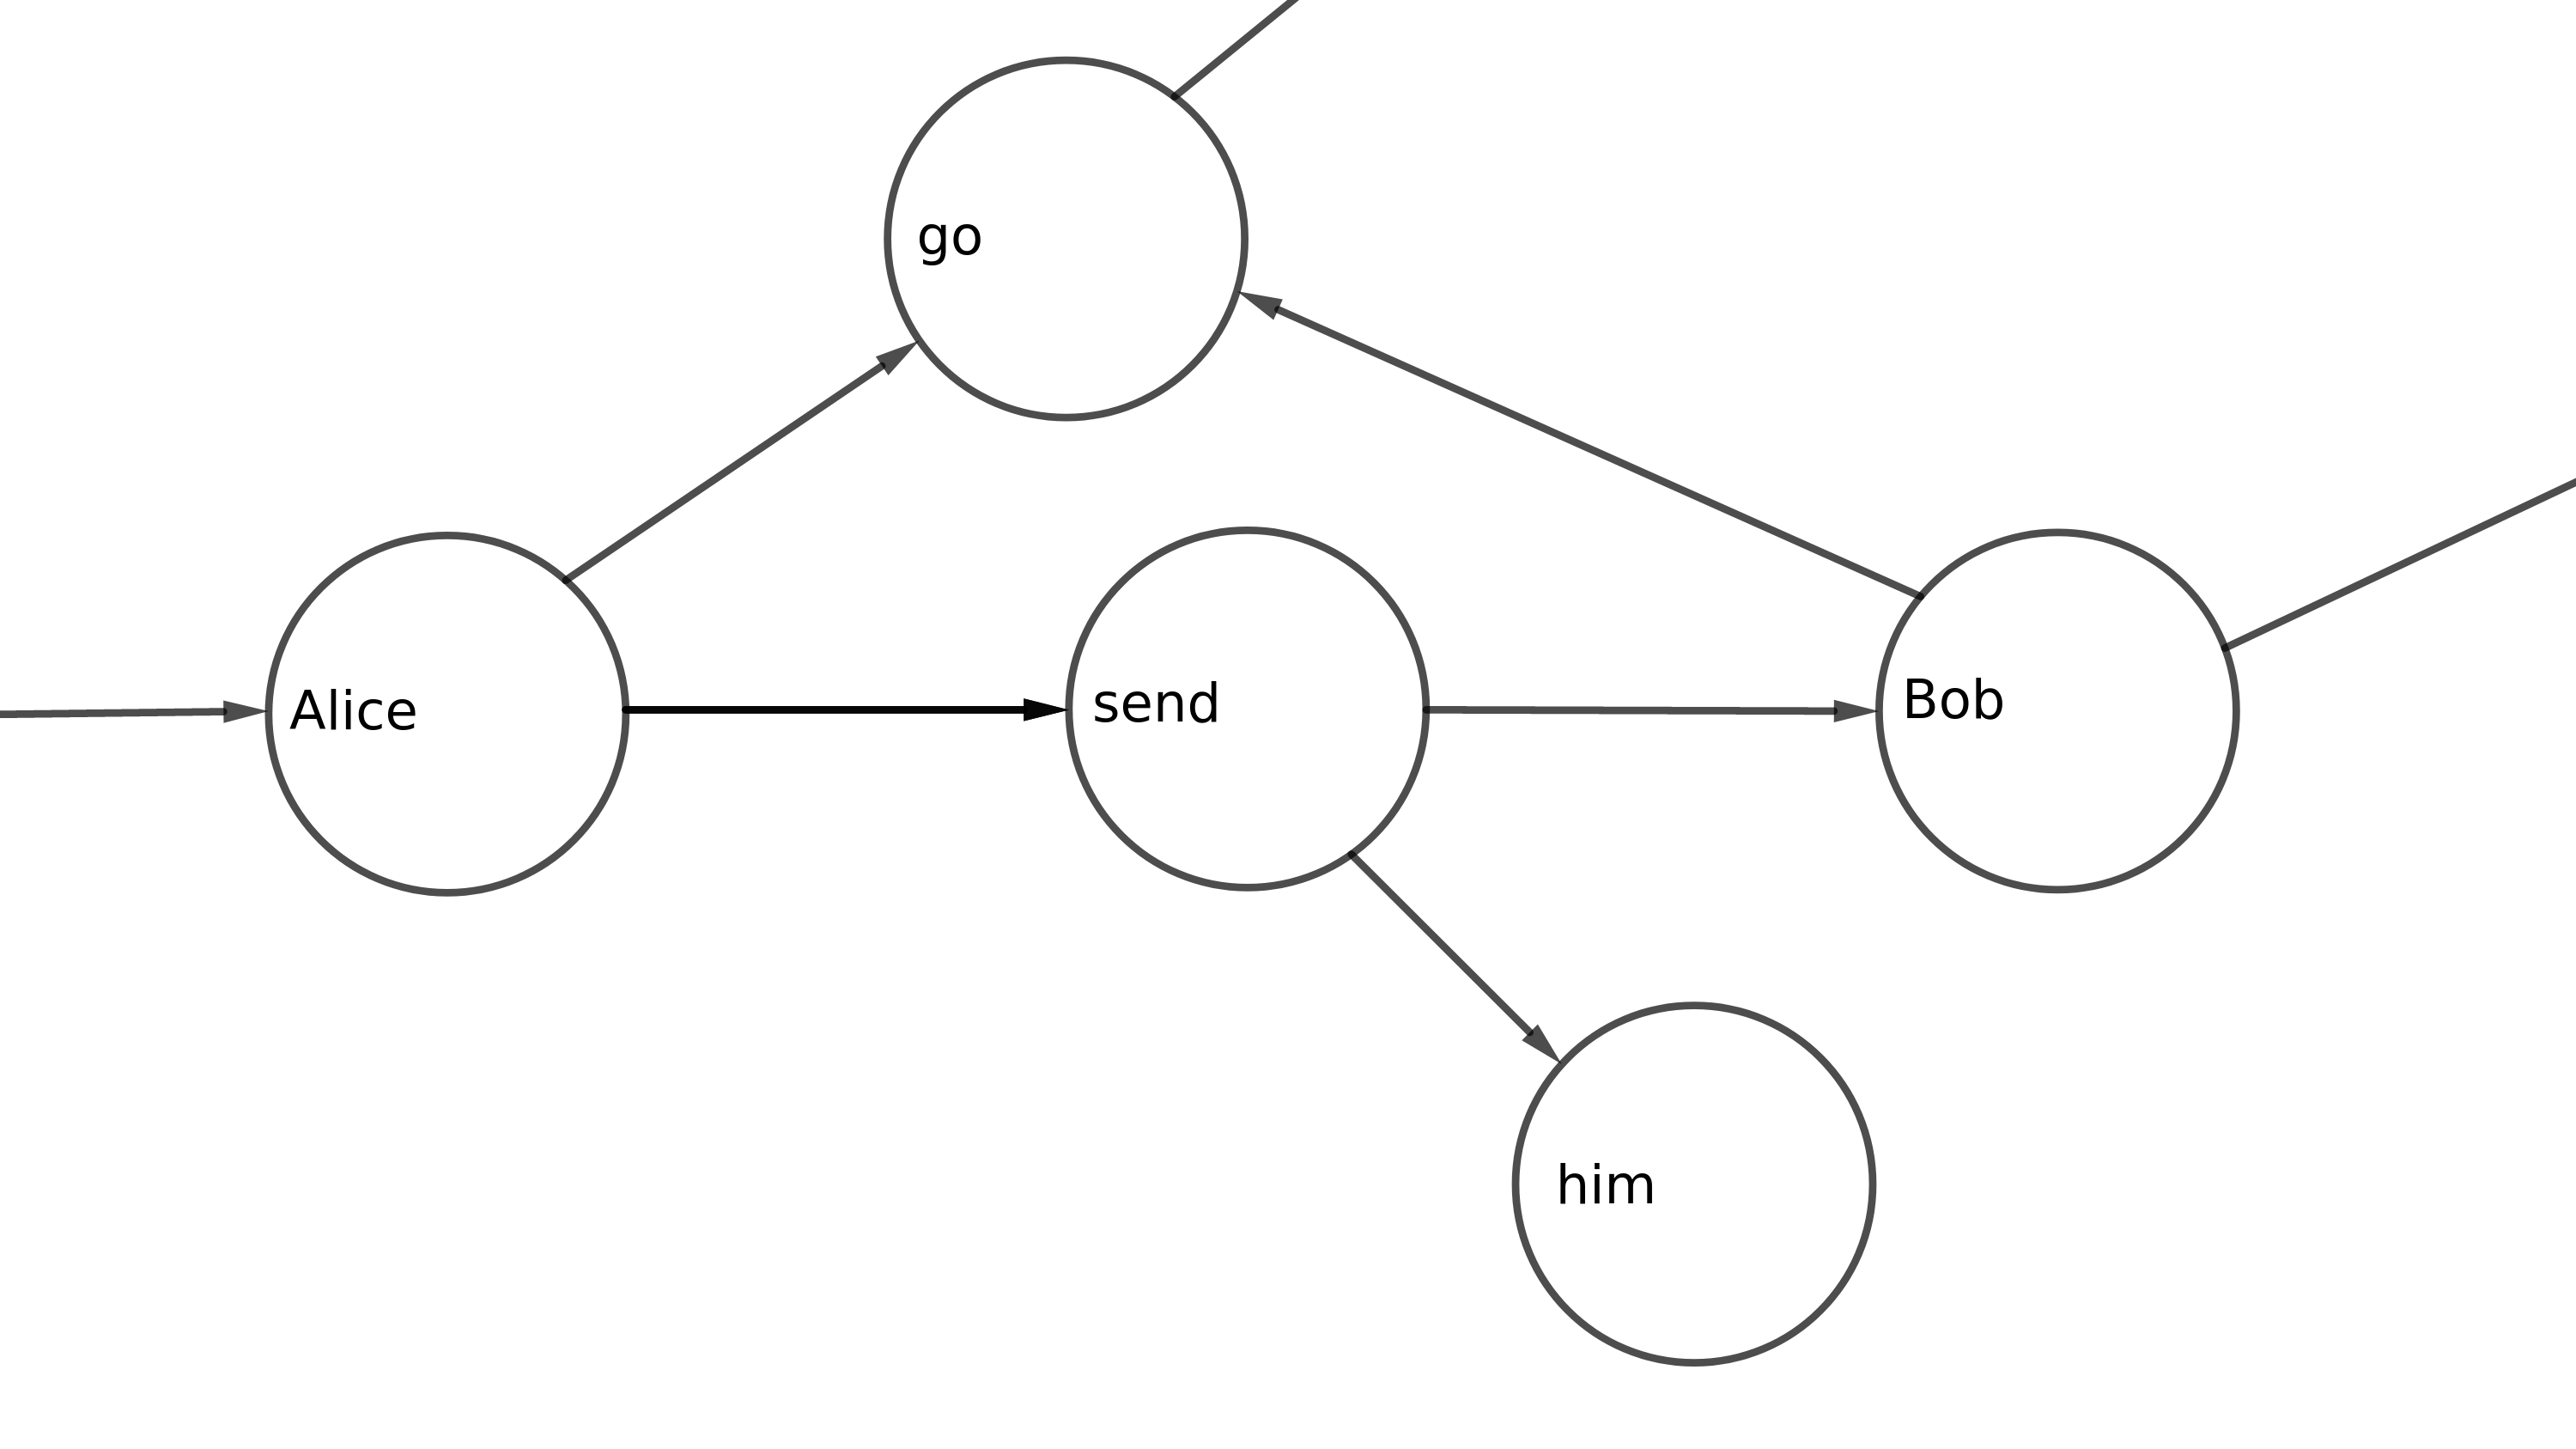
\includegraphics[scale=0.39]{Bilder/w2w_big}
			\end{figure}
		\end{column}
	\end{columns}
% --------------------------------------
\mynote{
	\begin{itemize}
		\item In the next steps more and more rules are added
	\end{itemize}
}
\end{frame}

% === OHE AND W2V ===================================

\begin{frame}
\frametitle{Word to word flavors}
\framesubtitle{\onehot{s} \& Word vectors}
	\begin{itemize}
		\item<1-> Word to word models come in two flavors
		\begin{itemize}
			\item<2-> \onehot{s} and
			\item<3-> Word vectors
			\item[] % Direkt einblenden, damit man nicht 2-3x weiterklicken muss
		\end{itemize}
	\end{itemize}
	\begin{columns}
		% SPALTE 1
		\begin{column}{0.375\textwidth}
			\begin{itemize}[leftmargin=15mm]
				\item<4-> Are $ 300d $ real valued vectors
				\item<5-> Potentially incorporate more information about a word
				\begin{itemize}
					\item<6->[$ \Rightarrow $] Better learning possible?
				\end{itemize}
				\item<7-> Probably the hippocampus receives multiple signals which are in total more related to word vector than to \onehot{}
				\begin{itemize}
					\item<8->[$ \Rightarrow $] Closer to reality
				\end{itemize}
			\end{itemize}
		\end{column}
		% SPALTE 2
		\begin{column}{0.625\textwidth}
			\begin{figure}
                \begin{overprint}
                    \centering
                        \includegraphics<1>[scale=0.39]{Bilder/w2w_big}
                        \includegraphics<2>[scale=0.39]{Bilder/w2w_ohe_big}
                        \includegraphics<3->[scale=0.39]{Bilder/w2w_w2v_big}
                \end{overprint}
			\end{figure}
		\end{column}
	\end{columns}
\mynote{
\begin{itemize}
    \item[ü] KEINE ÜBERLEITUNG
    \item word to word models come in two flavors
    \begin{itemize}
        \item equipped with \onehot{s} and ...
        \item word vectors
    \end{itemize}
	\item Word vectors can be calculated with \texttt{spacy} and are $ 300d $ real valued vectores as indicated in the graph
	\item They potentially incorporate more information about a word, STICHPUNKT EINBLENDEN therefore we hope they increase learning quality.
	\item Probably the hippocampus receives multiple signals which are in total more related to word vector than to \onehot{} STICHPUNKT EINBLENDEN
\end{itemize}
}
\end{frame}

% === AVERAGE APPROACH ===================================

% TODO Die anderen Konfigurationen erwähnen, am besten auf neue Folie
\begin{frame}[label={frame: average approach}]{Word to word Models}{Average approach}
	\begin{itemize}
		\item<+-> Predicting all instances of a word class at once and average the result (into one vector)
		\item<+-> Word classes are inferred by {\huge \texttt{spacy}}, $ 10 $ in total are used
		\item<+-> Idea: Meta word pairs like {\huge \texttt{Pronoun → Verb}} appear more frequently than {\huge \texttt{he → plays}}
		\item<+-> Averaging is done with both vector types: \onehot{s} and word vectors
	\end{itemize}
% --------------------------------------
\mynote{
\begin{itemize}
    \item[ü] There is also an average approach for word to word models
	\item It works by predicting all instances of a word class at once and average the result (into one vector)
	\item The word classes of the $ 10 $ highest indices are inferred by {\huge \texttt{spacy}}
	\item The idea behind averaging was that meta word pairs like {\huge \texttt{Pronoun → Verb  (Pronoun followed by Verb)}} appear more frequently than {\huge \texttt{he → plays (he then plays)}}, so a coarser tool may be worth trying
	\item The Averaging takes place for both vector types: \onehot{s} and word vectors
\end{itemize}
}
\end{frame}